% LTeX: language=en-GB
% !TeX root = ..\Thesis.tex
\section{Design}\label{sec:04}
The design of SteelBrew will take an Agile approach to get going with some framework for writing and running simple tests on devices written in SystemVerilog, using Java.
\subsection{Use cases}
Using SteelBrew should be as simple as possible. \cref{fig:usecases} shows an overview of the use cases for a developer.
\begin{figure}
    \centering
    \caption{Use case diagram for SteelBrew}\label{fig:usecases}
    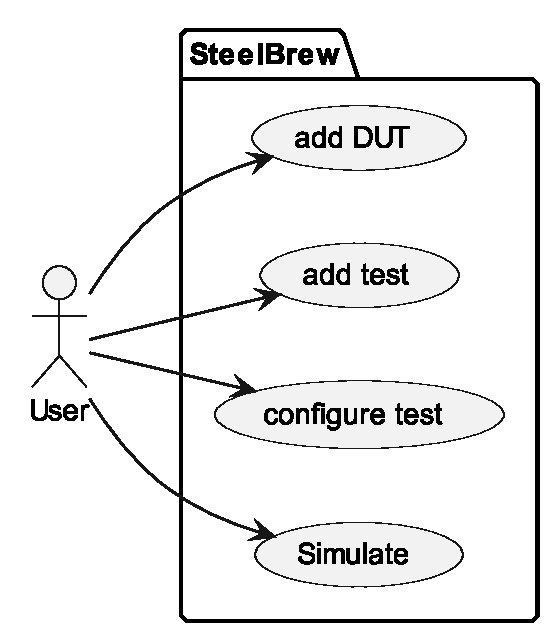
\includegraphics[width=.3\textwidth]{out/plantuml/usecase/usecase.eps}
\end{figure}
This is a simplification. As mentioned the framework is executed in Java, so to get started the user would start by creating a java project and importing SteelBrew. Hereafter the DUT is added and tests are defined and configured. A command should then execute the test and start the simulation.
\subsubsection{Adding the device under test}
With the device design in the root folder, adding it to the framework should be as easy as adding the device to some object that handles device configuration. The underlying logic should take care of the rest.
\subsubsection{Adding tests}
Since the tests are linked to some device, it is preferred that the same underlying logic ties tests and devices.
\subsubsection{Configure tests}
This is the bulk of the interaction for the user. With some object carrying the tests and device, the user should be able to easily add new tests or assertions with some easy to use method calls. The underlying logic should resolve conflicts and handle test creation without the user getting much involved.
\subsubsection{Simulate}
Since the simulations are carried out by a third-party program, all handling between SteelBrew and said program, should be handled by yet another class, separate from the test-driven class. This ensures good separation of responsibility in the project.
\subsection{Separation of responsibility}
The project is considered two-fold:
\begin{enumerate}
    \item Handling DUT's and tests
    \item Handling concurrency and third-party software
\end{enumerate}
For this reason the program has to contain two main components. The \emph{Brewer} and the \emph{Forge}.
A third class is introduced as the entry-point for the program, and will be accessible to all other classes. This class is simply \emph{SteelBrew}.
Expanding on \cref{fig:usecases}, the use case diagram is expanded as seen on \cref{fig:usecases2}.
\begin{figure}
    \centering
    \caption{The expanded use case diagram for SteelBrew}\label{fig:usecases2}
    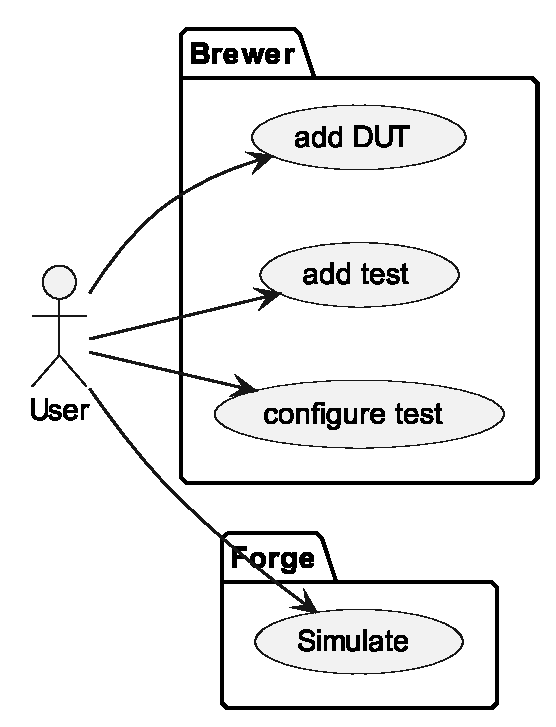
\includegraphics[width=.3\textwidth]{out/plantuml/usecase2/usecase2.eps}
\end{figure}
\subsection{The Brewer}
The Brewer is the primary interface. There are several ways of going about this object handling multiple DUT's and tests. One aspect could be to hold Lists or Maps of the tests and devices, and then use methods to get these, and couple them accordingly. This have the advantage that from a schematic point of view it simplifies the program. However, once tests are applied to different devices, all contained within the same object, one has to keep track of internal links. The first major decision in the design phase was as such:
\begin{enumerate}
    \item Give a Brewer to each DUT
    \item Assign tests to each Brewer
\end{enumerate}
This means more objects are created, but the Brewer object itself has a lot less responsibility in terms of tracking the interal links.\newline
A squence diagram on \cref{fig:seqBrew} shows this initial idea.
\begin{figure}
    \centering
    \caption{Sequence diagram showing the idea behind the Brewer}\label{fig:seqBrew}
    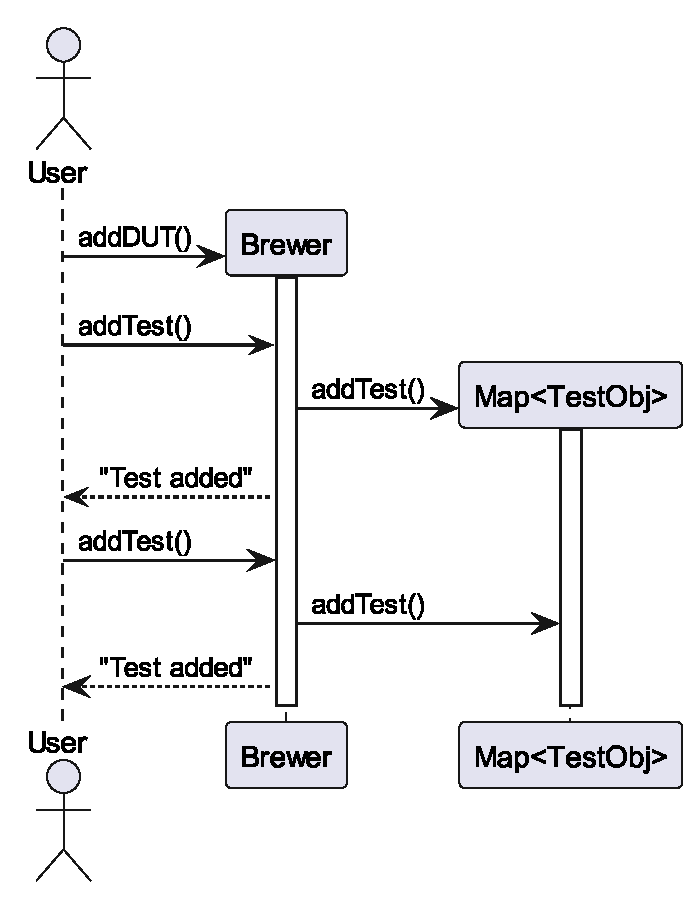
\includegraphics[width=.3\textwidth]{out/plantuml/Brewer/brewer.eps}
\end{figure}
\subsection{The Forge}
The Brewers complement, the Forge handles another job, entirely. This class has to handle the responsibility of taking the tests from the Brewers and hand them down to the third-party tool. This prompts some considerations, namely how to launch other programs with very specifik parameters and how to communicate with these programs.
\subsubsection{Verilator and the Forge}
The third-party software chosen is Verilator. It is opensource and very quick at executing simulations. Verilator works like this:
\begin{enumerate}
    \item The user prepares testbenches describing the testing environment and the tests
    \item Verilator takes the testbench and some DUT as input and makes the files for compiling a C++ program
    \item Compiling and running the program executes the tests and outputs a waveform-file, which can be inspected by e.g. GTKWave.\footnote{GTKWave on the web: \href{https://gtkwave.sourceforge.net/}{gtkwave.sourceforge.net}}
\end{enumerate}

This puts constrains on the design of the program. The Forge needs to call Verilator multiple times and then needs to run the compiled program. To ease this, the program creates a Makefile and executes through this. Simple redirects of stdout means that the Forge can collect the output from Verilator and the simulation. 
\subsubsection{Concurrency}
Up until now the main idea was to take a Brewer pointing to a DUT, add some tests and then hand it off to the Forge for Verilating, compiling and running the simulation. This poses one issue: This way of evaluating the program means that tests can only be parralised in terms of Verilator's internal multithreading, and then one DUT with all it's test per thread. Verilator's internal multithreading is outside the scope of this project, so the only options is to get creative with the way tests are run. Normally when using Verilator, one testbench with all testing is run per DUT. The design choice here was to split up the tests, such that each test, or set of tests, gets its own testbench and its own compiled program. This way tests can be carried out in parralel by launching each workflow on different threads.
\subsubsection{Coroutines}
It was of great interest to involve coroutines in the project. Java does not support coroutines natively so workarounds were investigated. To this end, it turns out most coroutine frameworks and plugins are 6+ years old. They do not support newer Java versions, and thus not newer Java functionality. The design choice here was to use threads to execute tests.
\subsection{Testbench}
The workflow of Verilator and the design choice of splitting up tests into separate executables meant that the definition of tests were somewhat straightforward. The Brewer would have Testbench objects. Whenever tests are defined they are added to this object, and just before simulation, testbench files are created based on the content of the object. The testbenches have to have unique names, otherwise the Verilator executable and GNU Make will be unable to execute the correct benches.
\subsection{Batch}
While the Testbench class is able to contain all tests put in, it is basically a collection of strings. Furthermore, it is often desireable to control the sequence in which tests are executed, as the result from one test might affect the other. Or if one has to test what happens when manipulating signals inside the DUT. A new class is introduced to handle a sequence of tests, along with logic transforming simple methods into cumbersome strings for the testbench. The Batch class keeps a record of signals and tests involved in some scenario and when ready, creates a testbench with these tests executed as they are added by the user.
\subsection{Assertions}